%% ****** Start of file aiptemplate.tex ****** %
%%
%%   This file is part of the files in the distribution of AIP substyles for REVTeX4.
%%   Version 4.1 of 9 October 2009.
%%
%
% This is a template for producing documents for use with 
% the REVTEX 4.1 document class and the AIP substyles.
% 
% Copy this file to another name and then work on that file.
% That way, you always have this original template file to use.

\documentclass[aip,apl,preprint,a4paper]{revtex4-1}
%\documentclass[aip,reprint]{revtex4-1}
\usepackage{graphicx}% Include figure files
\usepackage{dcolumn}% Align table columns on decimal point
\usepackage{bm}% bold math
\draft % marks overfull lines with a black rule on the right
\def\SP#1{\textsuperscript{#1}}
\def\SB#1{\textsubscript{#1}}
\begin{document}

% Use the \preprint command to place your local institutional report number 
% on the title page in preprint mode.
% Multiple \preprint commands are allowed.
%\preprint{}

\title{Low Driving Voltage Band-filling-based III-V-on-Silicon Electroabsorption Modulator} %Title of paper

% repeat the \author .. \affiliation  etc. as needed
% \email, \thanks, \homepage, \altaffiliation all apply to the current author.
% Explanatory text should go in the []'s, 
% actual e-mail address or url should go in the {}'s for \email and \homepage.
% Please use the appropriate macro for the type of information

% \affiliation command applies to all authors since the last \affiliation command. 
% The \affiliation command should follow the other information.

\author{Qiangsheng Huang}
%\email[]{huangqiangsheng@zju.edu.cn}
%\homepage[]{Your web page}
%\thanks{}
%\altaffiliation{}
\affiliation{Centre for Optical and Electromagnetic Research, Zhejiang Provincial Key Laboratory for Sensing Technologies, Zhejiang University, Hangzhou, 310058, China}
\affiliation{Photonics Research Group, Department of Information Technology, Ghent University-IMEC, Ghent B-9000, Belgium}

\author{Yingchen Wu}
\affiliation{Photonics Research Group, Department of Information Technology, Ghent University-IMEC, Ghent B-9000, Belgium}
\affiliation{State Key Laboratory of Modern Optical Instrumentation, Centre for Integrated Optoelectronics, Department of Optical Engineering, Zhejiang University, Hangzhou, China 310027}

\author{Keqi Ma}
\affiliation{Centre for Optical and Electromagnetic Research, Zhejiang Provincial Key Laboratory for Sensing Technologies, Zhejiang University, Hangzhou, 310058, China}

\author{Jianhao Zhang}
\affiliation{Centre for Optical and Electromagnetic Research, Zhejiang Provincial Key Laboratory for Sensing Technologies, Zhejiang University, Hangzhou, 310058, China}

\author{Weiqiang Xie}
\affiliation{Photonics Research Group, Department of Information Technology, Ghent University-IMEC, Ghent B-9000, Belgium}

\author{Xin Fu}
\affiliation{Centre for Optical and Electromagnetic Research, Zhejiang Provincial Key Laboratory for Sensing Technologies, Zhejiang University, Hangzhou, 310058, China}
\affiliation{Photonics Research Group, Department of Information Technology, Ghent University-IMEC, Ghent B-9000, Belgium}

\author{Yaocheng Shi}
\affiliation{Centre for Optical and Electromagnetic Research, Zhejiang Provincial Key Laboratory for Sensing Technologies, Zhejiang University, Hangzhou, 310058, China}

\author{Kaixuan Chen}
\affiliation{ZJU-SCNU Joint Research Center of Photonics, Centre for Optical and Electromagnetic Research, South China Academy of Advanced Optoelectronics, Science Building No.5, South China Normal University, Higher-Education Mega-Center, Guangzhou 510006, China}

\author{Jian-Jun He}
\affiliation{State Key Laboratory of Modern Optical Instrumentation, Centre for Integrated Optoelectronics, Department of Optical Engineering, Zhejiang University, Hangzhou, China 310027}

\author{Dries Van Thourhout}
\affiliation{Photonics Research Group, Department of Information Technology, Ghent University-IMEC, Ghent B-9000, Belgium}

\author{Gunther Roelkens}
\affiliation{Photonics Research Group, Department of Information Technology, Ghent University-IMEC, Ghent B-9000, Belgium}

\author{Liu Liu}
\email{liu.liu@coer-scnu.org}
\affiliation{ZJU-SCNU Joint Research Center of Photonics, Centre for Optical and Electromagnetic Research, South China Academy of Advanced Optoelectronics, Science Building No.5, South China Normal University, Higher-Education Mega-Center, Guangzhou 510006, China}

\author{Sailing He}
\email{sailing@kth.se}
\affiliation{Centre for Optical and Electromagnetic Research, Zhejiang Provincial Key Laboratory for Sensing Technologies, Zhejiang University, Hangzhou, 310058, China}
\affiliation{ZJU-SCNU Joint Research Center of Photonics, Centre for Optical and Electromagnetic Research, South China Academy of Advanced Optoelectronics, Science Building No.5, South China Normal University, Higher-Education Mega-Center, Guangzhou 510006, China}
% Collaboration name, if desired (requires use of superscriptaddress option in \documentclass). 
% \noaffiliation is required (may also be used with the \author command).
%\collaboration{}
%\noaffiliation

\date{\today}

\begin{abstract}
In this paper, a new method for realizing a low driving voltage electroabsorption modulator based on the band-filling effect is demonstrated. The InP-based electroabsorption modulator is integrated using DVS-BCB adhesive bonding on a silicon-on–insulator waveguide platform. When the electroabsorption modulator is forward biased, the band-filling effect occurs, which leads to a blue shift of the exciton absorption spectrum while the absorption strength stays almost constant. In static operation, an extinction ratio of more than 20 dB with 100 mV bias variation is obtained in an 80 $\mu$m long device. In dynamic operation, 1.25 Gbps modulation with a 6.3 dB extinction ratio is obtained using only a 50 mV peak-to-peak driving voltage. The band-filling effect provides a novel method for realizing ultra-low-driving-voltage electroabsorption modulators.
\end{abstract}

%\pacs{}% insert suggested PACS numbers in braces on next line

\maketitle %\maketitle must follow title, authors, abstract and \pacs

% Body of paper goes here. Use proper sectioning commands. 
% References should be done using the \cite, \ref, and \label commands

Quantum-confined Stark effect (QCSE) based electroabsorption modulators (EAM) exhibit high speed, low energy consumption, relatively high extinction ratio and small footprint.\cite{Yong40,Fukano} These features make EAMs widely used in optical communications. In addition, the electroabsorption effect can also be used to build a high speed photodetector, which possesses a similar structure as that of an EAM.\cite{Welstand} This dual function property enables, e.g., on-chip optical transceivers \cite{Transceiver} and compact optoelectronic oscillators (OEO).\cite{Zhou} Recently, silicon photonics integrated with electronic devices fabricated in complementary (CMOS) production lines has become an enabling technology for the realization of integrated optical systems.\cite{Marpaung,Sun} High speed InP-based EAMs have also been successfully implemented in silicon photonic circuits though hybrid integration technology.\cite{Yong40,Transceiver,roelkensiii-v-on-silicon2015,fu52015} However, for silicon photonics, it is important to reduce the power consumption. Because the transition energy consumed by an EAM is proportional to the driving voltage squared,\cite{Yong40} a low driving voltage EAM is required in silicon photonics. On the other hand, an EAM directly driven by the low voltage swing signal from an advanced digital logical CMOS driver can also save the energy consumption from the electrical signal amplifier. Recently, sub-100 mV driving voltage silicon modulators based on a high Q microring resonator or a photonic crystal cavity have been demonstrated.\cite{Manipatruni,Shakoor:14} However, those devices are very sensitive to fabrication imperfections and cannot be used as photodetectors. For QCSE based EAMs, it is challenging to reduce the driving voltage without an increase in the modulator size and insertion loss. Even when using a complex slow-light Bragg waveguide to enhance light-matter interaction,\cite{gulow-voltage2013} it is still hard to integrate with silicon photonics and reduce the driving voltage to the level of silicon modulators. Therefore, it is desirable to find a new, simple way to reduce the driving voltage without requiring complex fabrication procedures.


The band-filling effect in modulation-doped multiple quantum-wells (MQWs) has been studied since 1980s.\cite{livescu1988free} The band-filling effect, whereby the conduction subbands are filled with a two-dimensional (2D) electron gas, results in a blue shift of the absorption edge. By controlling the bias voltage, the electron concentrations in the MQWs region can be adjusted. In this way, the MQWs absorption edge can be controlled by bias voltage through the band-filling effect. This effect, using modulation-doped quantum wells, has been exploited in 100 mV driven active Q-switching lasers.\cite{kalinovsky1993free} However, no EAM exploiting the band-filling effect has been demonstrated yet.


In this paper, we demonstrate a novel type of low driving voltage EAM based on the band-filling effect, operation at 1.55 $\mu$m. The EAM is bonded on and coupled to a silicon-on-insulator (SOI) waveguide circuit, which makes it attractive to be combined with a direct digital CMOS drive.


Fig.~\ref{fig:1} shows the cross-sectional view of the EAM integrated on SOI using DVS-BCB adhesive bonding technology.\cite{roelkensiii-v-on-silicon2015} It consists of a silicon ridge waveguide, a thin bonding layer and a III-V p-i-n diode. The 380 nm thick silicon ridge waveguide is etched 160 nm deep and planarized using SiO\SB{2}. The thin bonding layer includes a 30 nm thick DVS-BCB layer and 15 nm SiO\SB{2}. At the top of the III-V p-i-n structure, there is a 100 nm p++-InGaAs (1.5$\times$10\SP{19} cm\SP{-3}) layer allowing a low resistance metal contact. Below it, there is a 1.5 $\mu$m gradually-doped (2$\times$10\SP{18} to 1$\times$10\SP{18} cm\SP{-3}) p-InP. In the intrinsic region, a MQW stack is sandwiched between two separate confinement heterostructure layers (SCH) of In\SB{0.52}Al\SB{0.16}Ga\SB{0.32}As. The MQW stack (nominal photoabsorption edge at 1560 nm) consists of 10 compressively strained In\SB{0.65}Al\SB{0.09}Ga\SB{0.26}As quantum wells and 11 tensile strained In\SB{0.42}Al\SB{0.17}Ga\SB{0.39}As barriers. At the bottom of the III-V structure, a 150 nm thin n-InP (3$\times$10\SP{18} cm\SP{-3}) layer is present and also used as the lateral contact to the ground metal.  The detailed epitaxial layer structure is shown in Fig.~\ref{fig:1}(a) and (b).

\begin{figure}
	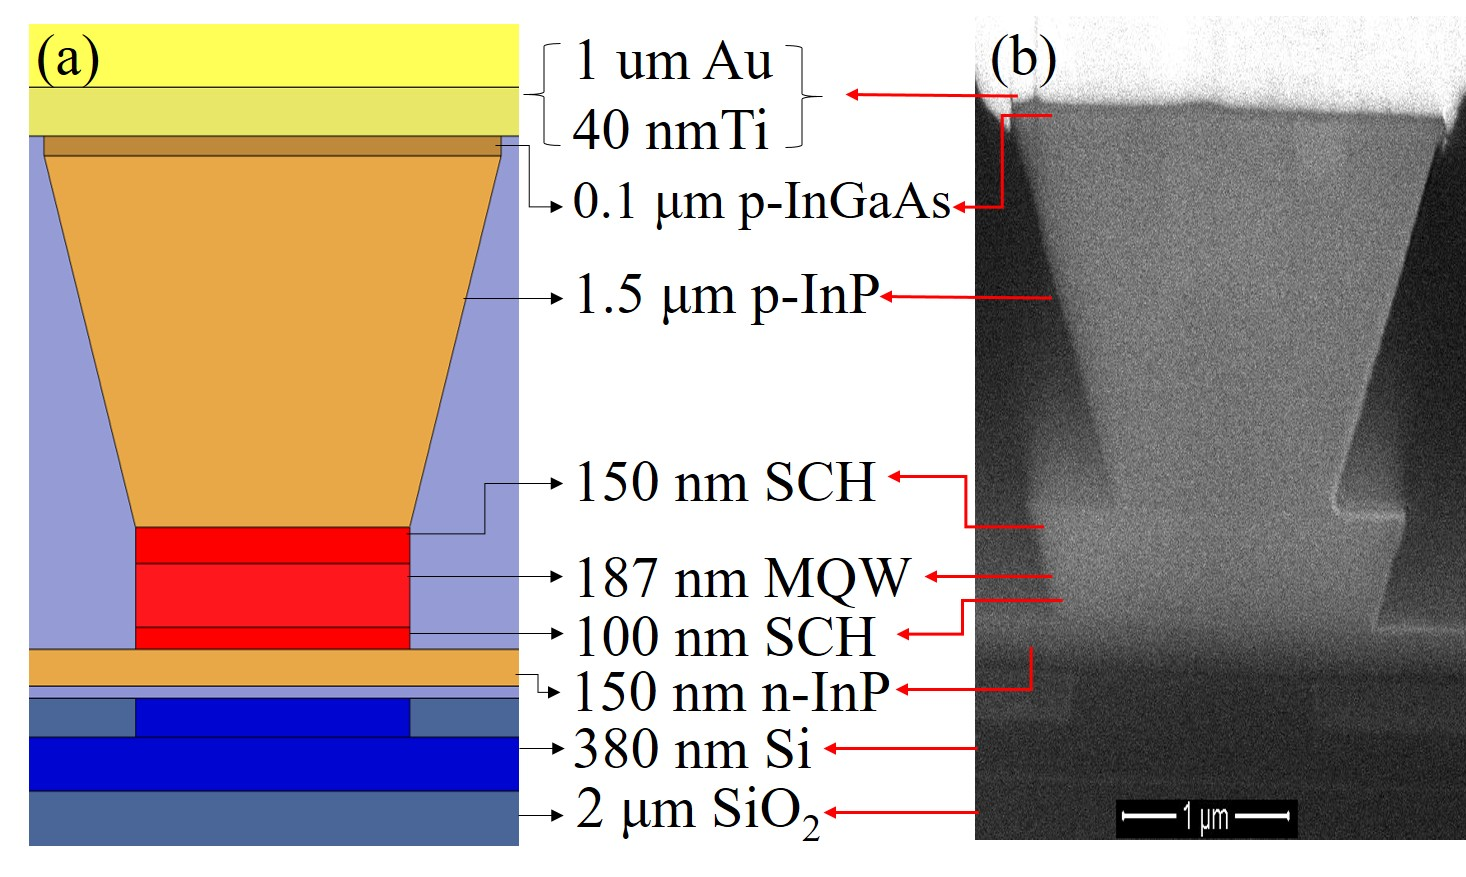
\includegraphics[width=6cm]{figure/fig1.eps}% Here is how to import EPS art
	\caption{\label{fig:1} (a) Cross-section view of the EAM bonded on SOI. (b) SEM image of the cross-section of the fabricated III-V/Si hybrid waveguide.}
\end{figure}

\begin{figure}
	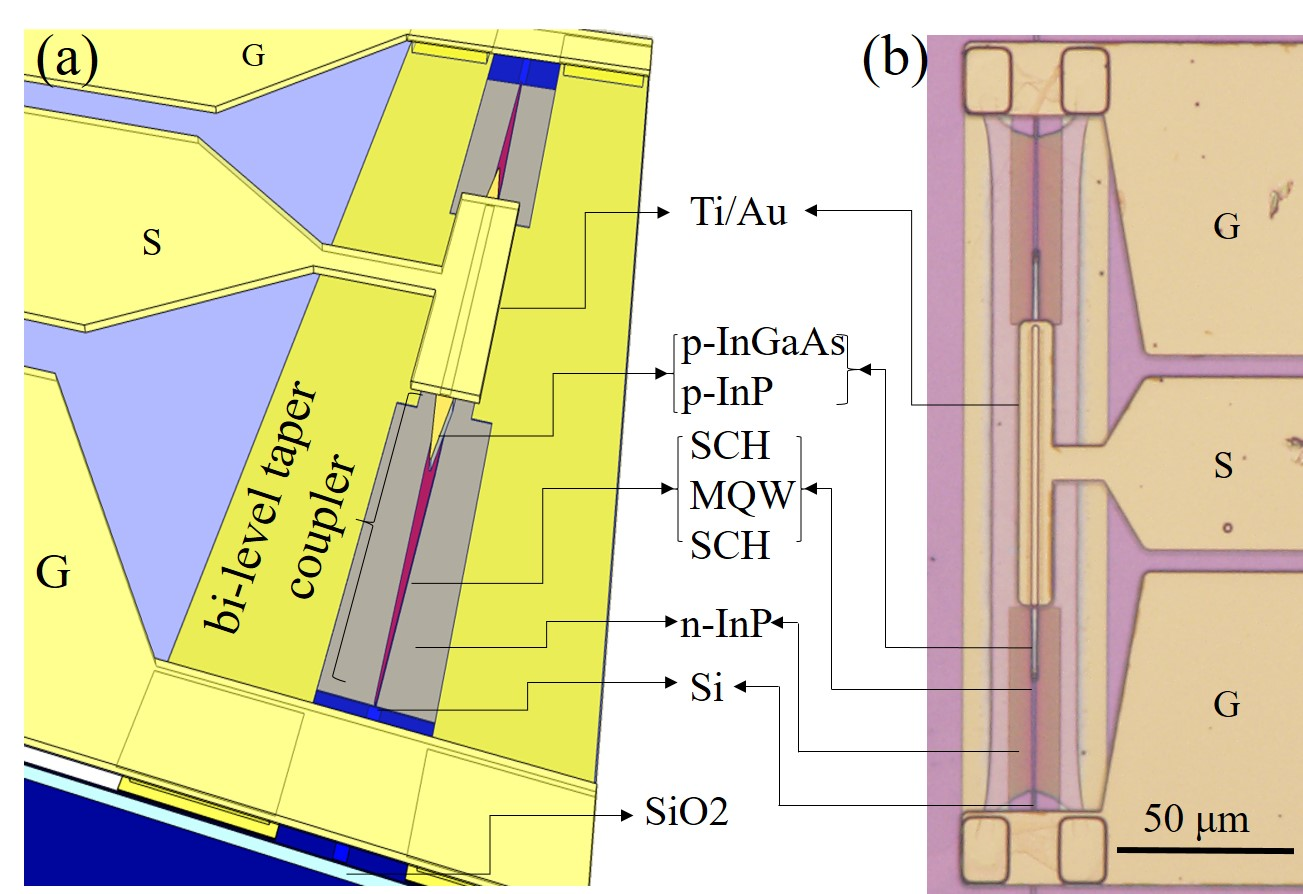
\includegraphics[width=6cm]{figure/fig2.eps}% Here is how to import EPS art
	\caption{\label{fig:2} (a) Three-dimensional sketch of the EAM bonded on SOI. (b) Top microscope image of the III-V/Si hybrid integrated EAM.}
\end{figure}


The fabrication process of this EAM is simpler than that of our previous laser/modulator.\cite{Transceiver,roelkensiii-v-on-silicon2015,fu52015} Thanks to the highly selective wet etching process used, a photoresist mask instead of a SiN hard mask can be used to define the III-V waveguide. In this way, the deposition and etching of SiN hardmask layers by PECVD and ICP-RIE respectively is avoided. The SOI waveguide circuit is fabricated through an ePIXfab Multi Project Wafer run.\cite{epixfab} The silicon ridge waveguide is 1.5 $\mu$m wide. After bonding and removing the InP substrate, the InGaAs layer is patterned by wet-etching (H\SB{3}PO\SB{4}:H\SB{2}O\SB{2}:H\SB{2}O = 1:1:20) using a photoresist mask. Then the p-InP waveguide is defined using the InGaAs pattern as a mask through wet etching (HCl:H\SB{2}O = 1:1). The waveguide cross section becomes an inverted trapezoid with a width of 2.5 $\mu$m at the top and 1.5 $\mu$m at the bottom. The MQW+SCH layers are patterned also with wet-etching (Citric:H\SB{2}O\SB{2} = 20:1) using a 5 $\mu$m wide photoresist mask.  By carefully controlling the amount of under-etching, the width of the MQW+SCH region is nominally reduced to 1.5 $\mu$m. A 0.1 $\mu$m thick Ni/Ge/Au alloy is deposited onto the n-InP forming the n-contacts. Then the n-InP is wet etched (HCl:H\SB{2}O = 1:1) in order to electrically isolate the devices. All the wet etching processes are performed at 20 $^{\circ}$C. A 2.5 $\mu$m thick DVS-BCB layer is used for passivation and planarization. Via holes are formed in the DVS-BCB for metal connections. Finally, a metal stack of 40 nm Ti/ 1 $\mu$m Au is deposited onto the p-InGaAs and n-contacts for forming the 100 $\mu$m pitch ground-signal-ground (GSG) metal contact. Fig.~\ref{fig:2}(a, b) respectively show the three-dimensional sketch of the designed lumped electrode EAM and a top-down photograph of a fabricated device. Fig.~\ref{fig:1}(b) shows the cross section of the fabricated III-V/Si hybrid waveguide structure.


The mode conversion from the silicon ridge waveguide to the hybrid waveguide is achieved by a 45 $\mu$m long bi-level taper in III-V material.\cite{fu52015,huang2015ultracompact} The silicon ridge waveguide remains 1.5 $\mu$m wide under the bi-level taper. In the first part of the taper, the mode is converted from the silicon ridge waveguide mode to that of the hybrid structure without the thick p-InP layer, where the MQW+SCH layers width laterally is tapered from 0.2 $\mu$m to 1.5 $\mu$m. The second part of the taper transforms the optical mode into that of the full III-V waveguide, where the p-InP layer is laterally tapered from 0.2 $\mu$m to 2.5 $\mu$m and the MQW+SCH layers are kept 1.5 $\mu$m wide. The simulated coupling efficiency between the silicon ridge waveguide and hybrid waveguide is around 98\%. The optical confinement factor in the ten quantum wells of the hybrid waveguide is around 24\%.


The present EAM with InAlGaAs MQWs exhibits a strong and sharp exciton absorption peak at the absorption edge due to its large conduction band offset.\cite{Fukano} Since the band-to-band continuum transition energy (which is above the exciton transition energy) has a small influence on the absorption edge, we adopt a theoretical model only containing the exciton transition, in order to simplify calculation of the absorption spectra and the shift of the absorption edge for the EAM.\cite{self‐electro‐optic‐effect} The material parameters of the MQW structure, such as the effective electron/hole mass, Luttinger parameters, band energy levels, etc., are taken from Ref. \onlinecite{li2000material}, taking into account the nominal composition of each layer. The half-linewidth for the absorption peak varies from 1 meV at zero electric field to 1.4 meV at 42 KV/cm, is taken from the measuring results. The effective mass m\SP{*} of the average matrix element is 0.0064 m\SB{0},\cite{self‐electro‐optic‐effect} where m\SB{0} is the electron mass. 


The simulated exciton absorption spectra for a 80 $\mu$m long EAM are shown in Fig.~\ref{fig:4}. Due to the p-i-n structure used, there is a built-in electric field at 0 V bias. Zero electric field in the intrinsic layer is achieved at a forward bias of 0.6 V. Below 0.6 V, the absorption spectra for the EAM are calculated using a QCSE model. The exciton absorption peak red shifts with increasing applied electric field. Due to the decreasing electron-hole overlap integral with increasing electric field, the absorption magnitude decreases. Above 0.6 V, the absorption spectra for the EAM are calculated using a the band-filling effect model. The exciton absorption peak blue shifts when more current is injected into the conduction band. Since the electron-hole overlap integral remains almost constant with increasing current density, the absorption does not decrease in magnitude. The exciton transition energy shift $\Delta E$ is given by: $\Delta E = (1+m_e/m_h)E_F$, where $E_F$ is the Fermi energy level for the electrons, and $m_e$ and $m_h$ are the effective electron and hole mass, respectively.\cite{livescu1988free} When $E_F$ is substantially higher than the lowest conduction subbands $E_1$, $E_F$ increases linearly as the carrier density  increases in the quantum well.\cite{Coldren} Since the carrier density is proportional to the injected current, and the injected current is directly related to the applied voltage, the absorption peak shift is directly proportional with the applied voltage. In this way, by modulating the applied voltage, we can build an efficient modulator.

\begin{figure}
	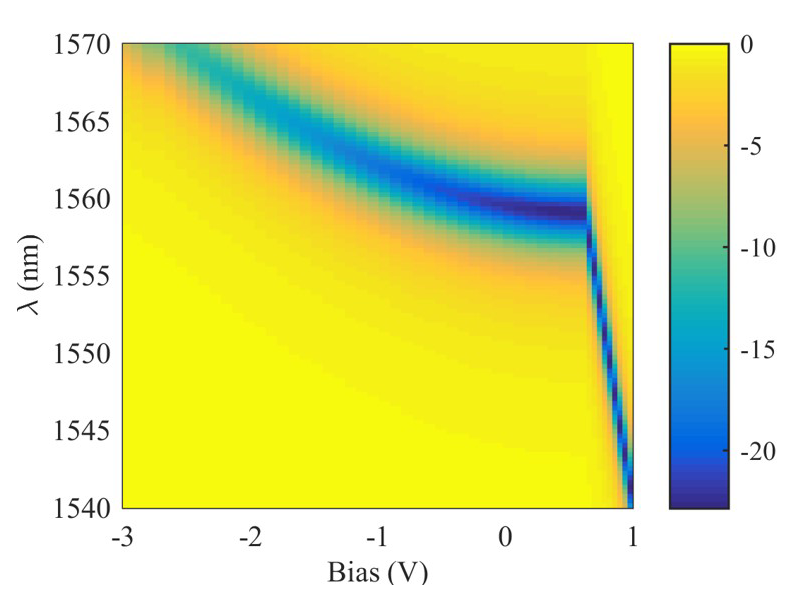
\includegraphics[width=6cm]{figure/fig4.eps}% Here is how to import EPS art
	\caption{\label{fig:4} The simulated exciton absorption spectra (dB) for the 80 $\mu$m long EAM with different bias voltages. The strongest absorption is more than 20 dB.}
\end{figure}


We first measure the EAM’s static performance as a function of bias at 1.55 $\mu$m, as shown in Fig.~\ref{fig:5}(a). The measurement results are normalized to the transmission through a straight waveguide using the same fiber-chip interface. The insertion loss of the EAM is around 5 dB at zero bias, larger than the simulation results. This is attributed to the fact that the width of the MQW+SCH region in the fabricated device is larger than the designed value of 1.5 $\mu$m, shown in Fig.~\ref{fig:1}(b). In this case, the bi-level taper coupler will excite higher order modes and cause unwanted reflection during mode transformation, especially in the first level taper.\cite{huang2015ultracompact} Fig.~\ref{fig:5}(a) shows that there are two regimes of absorption variation versus bias voltage. In reverse bias, the absorption variation is caused by continuum transition absorption (the classic electroabsorption effect). Due to the short device length, the extinction ratio is only around 4dB with the voltage changing from -1V to -2V. In forward bias, the absorption variation is caused by the exciton transition absorption. The change in absorption is more than 20 dB with only 100 mV bias variation. The measured absorption spectra with bias variation are shown in Fig.~\ref{fig:5}(b). The exciton peak absorption and shifts are in good agreement with the simulation results shown in Fig.~\ref{fig:4}. In the forward bias, the blue shift rate of the exciton absorption peak is around 50 nm/V, without a reduction in absorption strength. Therefore, a low driving voltage EAM can be realized in the forward bias.

\begin{figure}
	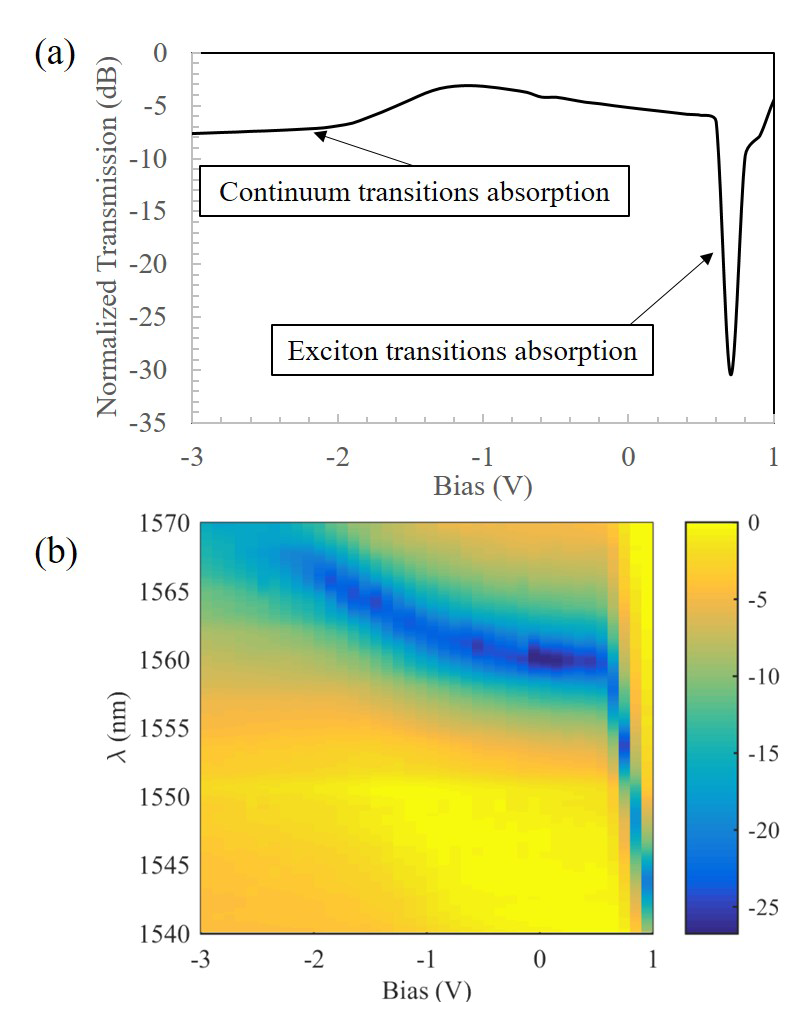
\includegraphics[width=8cm]{figure/fig5.eps}% Here is how to import EPS art
	\caption{\label{fig:5} (a) The bias dependent normalized transmission for the 80 $\mu$m long EAM at 1.55 $\mu$m. (b) The exciton absorption spectra (dB) for different bias voltages. The strongest absorption is more than 20 dB.}
\end{figure}

Next, we measure dynamic performance of the EAM at 1.55 $\mu$m. A non-return-to-zero (NRZ)  2\SP{31}-1 pseudorandom bit sequence (PRBS) pattern is generated and  attenuated  to  a  level  of  50 mV  swing,  and then  applied  to  the III-V-on-silicon EAM via a bias-T providing a forward bias of 0.6 V. The modulated light is coupled out to a fiber through a fiber-to-chip grating coupler and amplified by an erbium-doped fiber amplifier (EDFA). The amplified spontaneous emission generated by the EDFA is subsequently filtered out by a narrow optical filter. Eye diagrams are measured using a Tektronix 8300A digital series analyzer. The 1.25 Gbps eye diagram of the EAM is shown in Fig.~\ref{fig:6}(a). The dynamic extinction ratio is 6.3 dB, which is twice as large as the low voltage drive silicon modulators based on tuning the resonant wavelength with the same peak-to-peak voltage.\cite{Shakoor:14} The method to calculate the energy consumption of the EAM is presented in Ref. \onlinecite{Yong40}. Because the cross-section of our 80 $\mu$m long EAM is the same as our previous 100 $\mu$m long modulator,\cite{fu52015} the junction capacitance is estimated to be around 116 fF. The transient energy consumption for this EAM is 0.29 fJ/bit. The transient energy consumption can be further reduced by narrowing the MQW+SCH layer width, which effectively decreases the junction capacitance. The DC energy consumption per bit at 1.25 Gbps is 110 fJ/bit, which can be reduced by increasing the modulator speed. It is worthwhile noting that the rise and fall time is limited by the carrier lifetime in the MQWs for the present EAM working under a forward bias. Fig.~\ref{fig:6}(b) shows the high-speed performance for the same EAM working under a reverse bias at a data rate of 12.5 Gbps with a voltage swing of 1.1 V. One can see that the modulation bandwidth is significantly increased due to the fact that the carrier lifetime is largely reduced at a reverse bias. The speed of the EAM in this case is limited by the RC time constant.\cite{Yong40,fu52015} Using modulation-doped MQWs to move the Fermi energy level above the lowest confined state in the conduction band at zero bias, we can shift the working point to a reverse bias.\cite{livescu1988free,kalinovsky1993free} In this way, the modulation bandwidth of the present band-filling based EAM can also be increased.

\begin{figure}
	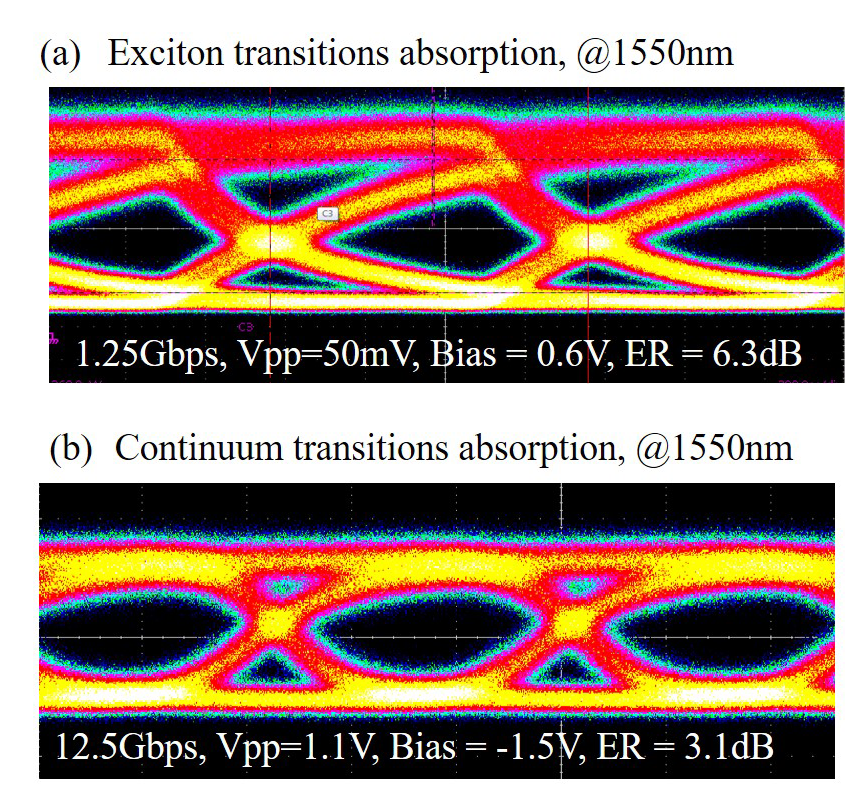
\includegraphics[width=6cm]{figure/fig6.eps}% Here is how to import EPS art
	\caption{\label{fig:6} Measured 2\SP{31}-1 PRBS NRZ eye diagrams at 1.55 $\mu$m (a) 1.25 Gbps at forward bias 0.6 V.  (b) 12.5 Gbps at reverse bias -1.5 V.}
\end{figure}


In summary, we have demonstrated an III-V-on-silicon EAM based on the band filling effect. With 100 mV bias variation, the DC extinction ratio is better than 20 dB. The exciton absorption peak shift and intensity variation are in good agreement with the simulation results. A clear open eye diagram has been obtained at 1.25 Gbps with a dynamic extinction ratio of 6.3 dB. The peak-to-peak driving voltage is only 50 mV. The speed of the present device is limited by carrier lifetime and can be further improved by using modulation-doped MQWs. The insertion loss and transient energy consumption can be further improved with optimized fabrication processes. 

% If you have acknowledgments, this puts in the proper section head.
\begin{acknowledgments}
This work was partially supported by the National Natural Science Foundation of China (91233208 \& 61377038), the National High-Tech R\&D Program of China (grant No. 2013AA014401), the Program of Zhejiang Leading Team of Science and Technology Innovation and the China Scholarship Council (award to Qiangsheng Huang, Yingchen Wu and Xin Fu for 1 year’s study abroad at Ghent University) and the European Commission through the ERC-project ULPPIC.
\end{acknowledgments}

% Create the reference section using BibTeX:
\bibliography{v1}

\end{document}
%
% ****** End of file aiptemplate.tex ******
